\section{Programm}
Wie in der Abbildung \ref{fig:meineSimulation} im Anhang zu sehen ist, werden in der Simulation die Elektronenkanone, die Ablenkspulen und der Bildschirm der Fernsehröhre animiert. 
Dabei kann die Spannung der Elektronenkanone gesteuert werden und die Magnetfeldstärke ebenfalls angepasst werden.
Dadurch wird die Geschwindigkeit der Elektronen des Strahls, die Ablenkung des Strahls und schlussendlich der Auftreffpunkt jeweils dynamisch neu berechnet.
In den groß dargestellten Kreisen ist die genaue Ablenkung des Strahls durch die einzelnen Ablenkfelder dargestellt, während aufgrund der Bildauflösung am Schnittpunkt $M$ der Magnetfelder diese kreisförmige Ablenkung nicht visualisiert werden kann.   
Deswegen wird dies, wie angemerkt, in den Kreisen oben separat dargestellt.\footnote{Diese Kreise entsprechen dem grauen Kreis in Abbildung \ref{fig:ausBlog}.}
Die Geschwindigkeit, welche in den Kreisen erscheint, entspricht nicht der wirklichen Geschwindigkeit der Elektronen, da diese zu hoch ist und dadurch nicht zu sehen wäre.
Die Umsetzung des Programms erfolgte in Java mit der Greenfoot-Umgebung.
\label{sec:animation}

\section{Berechnungen zur Elektronenkanone}

%\subsection{physikalische Erklärung:}
\label{sec:tolle-section}
 
Durch die Heizspannung wird die Kathode zum Glühen gebracht, wodurch Elektronen aus der Kathode austreten (glühelektrischer Effekt).
Die Elektronen haben zu Beginn eine Geschwindigkeit von etwa $0 \frac{m}{s}$.
Im homogenen elektrischen Feld zwischen Kathode (negativ) und Anode (positiv) werden die Elektronen beschleunigt.
Dadurch fliegen die Elektronen mit zunehmender Geschwindigkeit auf die Anode zu.
Dahin werden die Elektronen durch einen Wehnelt-Zylinder auf der Mittelachse konzentriert.
Wegen dieser Richtungsfokussierung sowie ihrer erreichten Geschwindigkeit "`fliegen"' die Elektronen durch die Annodenbohrung hindurch und kommen als gebündelter und sich geradlinig bewegender Elektronenstrahl aus der Elektronenkanone heraus.
Da die elektrische Energie in kinetische Energie umgewandelt wird, gilt laut dem Energieerhaltungssatz:
\begin{equation}
\label{eq:Energie}
   E_{kin} = E_{el}  
\end{equation}
$$ \frac{1}{2} \cdot m \cdot v^2 = e \cdot U_B$$
Diese Formel wird  nun nach $v$ umgestellt:
%\subsection{Die physikalische Formel:} 
\begin{equation}
\label{eq:v}
   v = \sqrt{\frac{2 \cdot e \cdot U_B}{m}} 
\end{equation}
%\subsection{Erklärung/Umsetzung der Physik im Code:}

Im Folgenden ist ein kurzer Auszug des Codes der Simulation dargestellt.
Zu sehen ist, dass die oben genannte Formel (\ref{eq:v}) benutzt wird und die jeweiligen Attribute aus den zugehörigen Klassen geholt werden.
Dabei wird die Spannung $U_B$ aus der Programmklasse Elektronenkanone (Objekt \lstinline$quelle$) gelesen.

\begin{lstlisting}
teilchengeschwindigkeit 
  = Math.sqrt(2 * elektronenladung * quelle.spannung * 1000 
              / elektronenmasse);
\end{lstlisting}
Die Multiplikation mit 1000 findet statt, da die Spannung im Programm in Kilovolt gespeichert wird (siehe Anhang \ref{sec:Appendix}).
\section{Lorentzkraft und Ablenkung}
\label{sec:a}
%\subsection{physikalische Erklärung:}

Das Magnetfeld der Ablenkspulenpaare ist homogen und steht jeweils senkrecht zu der Bewegungsrichtung der Elektronen.
Die Elektronen kommen mit einer gewissen Geschwindigkeit $v$ aus der Elektronenkanone heraus und diese bleibt auch im weiteren Verlauf konstant.
Die Lorentzkraft $F_L$ wirkt stets senkrecht zur Bewegungsrichtung der Elektronen und der Betrag der Geschwindigkeit bleibt dadurch konstant.
Hier lässt sich die Lorentzkraft als Zentripetalkraft auffassen, da die Elektronen somit auf eine Kreisbahn abgelenkt werden (wobei der Radius dieser Kreisbahn im nächsten Abschnitt für die Berechnung der Ablenkung gebraucht wird).
Wie bereits beschrieben, wirkt die Lorentzkraft als Zentripetalkraft immer senkrecht auf die Bewegungsrichtung der Elektronen.
Dies bedeutet, dass die Kraftkomponente in Bewegungsrichtung nicht vorhanden ist und die Geschwindigkeit deswegen konstant bleibt.
Durch den Kraftansatz leitet sich ab: 
\begin{equation}
\label{eq:Kraft}
   F_L=F_z 
\end{equation}
$$ e \cdot v \cdot B = \frac{m \cdot v^2}{r}$$
Dies lässt sich nun nach $r$ umstellen und man erhält die folgende Formel.   

%\subsection{Die physikalische Formel:}

\begin{equation*}
     r = \frac{m \cdot v}{e \cdot B}
\end{equation*}

\section{Geometrische Bestimmung des Auftreffspunktes auf dem Schirm}
\label{sec:g}
Die folgenden geometrischen Erklärungen orientieren sich an \cite{Blog} und \cite{Gente1950}.
%\subsection{geometrische Erklärung:}

Die Situation ist wie in der Abbildung \ref{fig:ausBlog} dargestellt.\footnote{Eine ähnliche Abbildung befindet sich auf Seite 16 von \cite{Gente1950}.}
Um geometrisch den Ablenkwinkel zu berechnen, wird die Annahme getroffen, dass die Ablenkung des Magnetfeldes nur in einem kreisförmigen Ausschnitt wirkt.
Aus der Skizze ergibt sich, dass der Ablenkwinkel, um den der Strahl geknickt wird, gleich ist zu dem Winkel im großen Kreis zwischen den Punkten A (Eintrittspunkt in den kleinen Kreis) und B (Austrittspunkt aus dem kleinen Kreis).
Im rechtwinkligen Dreieck aus dem Punkt A und den beiden Mittelpunkten der Kreise kann man die Definition des Tangens benutzen.
Der Winkel ist $\frac{\alpha}{2}$, da die Winkelhalbierende als Verbindungslinie fungiert.
Also gilt die Formel:
\begin{equation}
    \label{eq:tan}
    \tan \left(\frac{\alpha}{2}\right) = \frac{d}{2}:r = \frac{d}{2 \cdot r}
\end{equation}
Um festzustellen, in welche Richtung um den Winkel $\alpha$ abgelenkt wird, müssen die Richtungsvektoren des Strahls und des Magnetfeldes betrachtet werden.
Die Lorentzkraft wirkt in die Richtung des Kreuzprodukts dieser beiden.
Da mit negativen Teilchen gearbeitet wird, muss der Richtungsvektor des Strahls umgedreht werden. Dadurch ergibt sich die Formel: \begin{equation}
    \label{eq:a}
    \vv{a} = - \vv{s}\times \vv{b}
\end{equation}
Um den Endpunkt auf dem Schirm zu bestimmen, kann die Skizze aus Abbildung \ref{fig:Schirm} zu Hilfe genommen werden.
Der Punkt $M$ stellt den Mittelpunkt des kleinen Kreises aus der Abbildung \ref{fig:ausBlog} dar.
Der Punkt $E$ stellt den Punkt dar, wo der Strahl auf den Schirm trifft.
Der Punkt $U$ hingegen stellt den Mittelpunkt des Schirms dar.
Der Winkel $\alpha$ stellt den Winkel dar, welcher sich aus der Formel (\ref{eq:tan}) ergibt und $\vv{a}$ stellt die Ablenkrichtung des Strahls dar, welche mit der Formel (\ref{eq:a}) berechnet wurde.
Da man ein rechtwinkliges Dreieck hat, kann man die Länge ausrechnen, welche die Seite $\vv{UE}$ hat.
Dies entspricht einem Vektor $\vv{v_\mathit{diff}}$, welchen man zum Ortsvektor von $U$ addieren kann.
Die Formel ist:
\begin{equation}
    \label{eq:v_d}
    \vv{v_\mathit{diff}} =  \vv{a} \cdot l \cdot \tan(\alpha)
\end{equation}
Da mit zwei Spulenpaaren gearbeitet wird, müssen die Formeln (\ref{eq:tan}), (\ref{eq:a}) und (\ref{eq:v_d}) jeweils zweimal wiederholt werden.
Nun ist der Vektor $\vv{v_\mathit{diff}}$ zweimal vorhanden, einmal für das senkrechte und einmal für das waagerechte Magnetfeld.
Diese beiden Vektoren werden auf den Punkt $U$ (Ortsvektor) hinzuaddiert, sodass sich der endgültige Punkt $E$ ergibt.
\begin{figure}
    \centering
    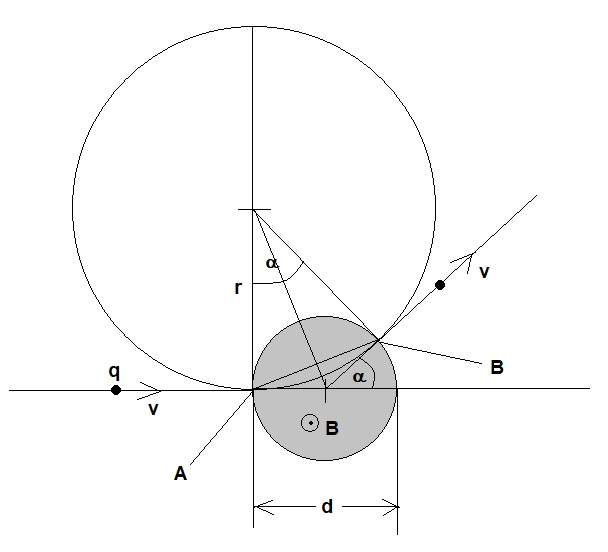
\includegraphics[width=.75\textwidth]{fig/elektronenstrahl-ablenkung_101.jpg}
    \caption{Skizze für Winkelberechnung (übernommen von \cite{Blog})}
    \label{fig:ausBlog}
\end{figure}

\begin{figure}
    \centering
    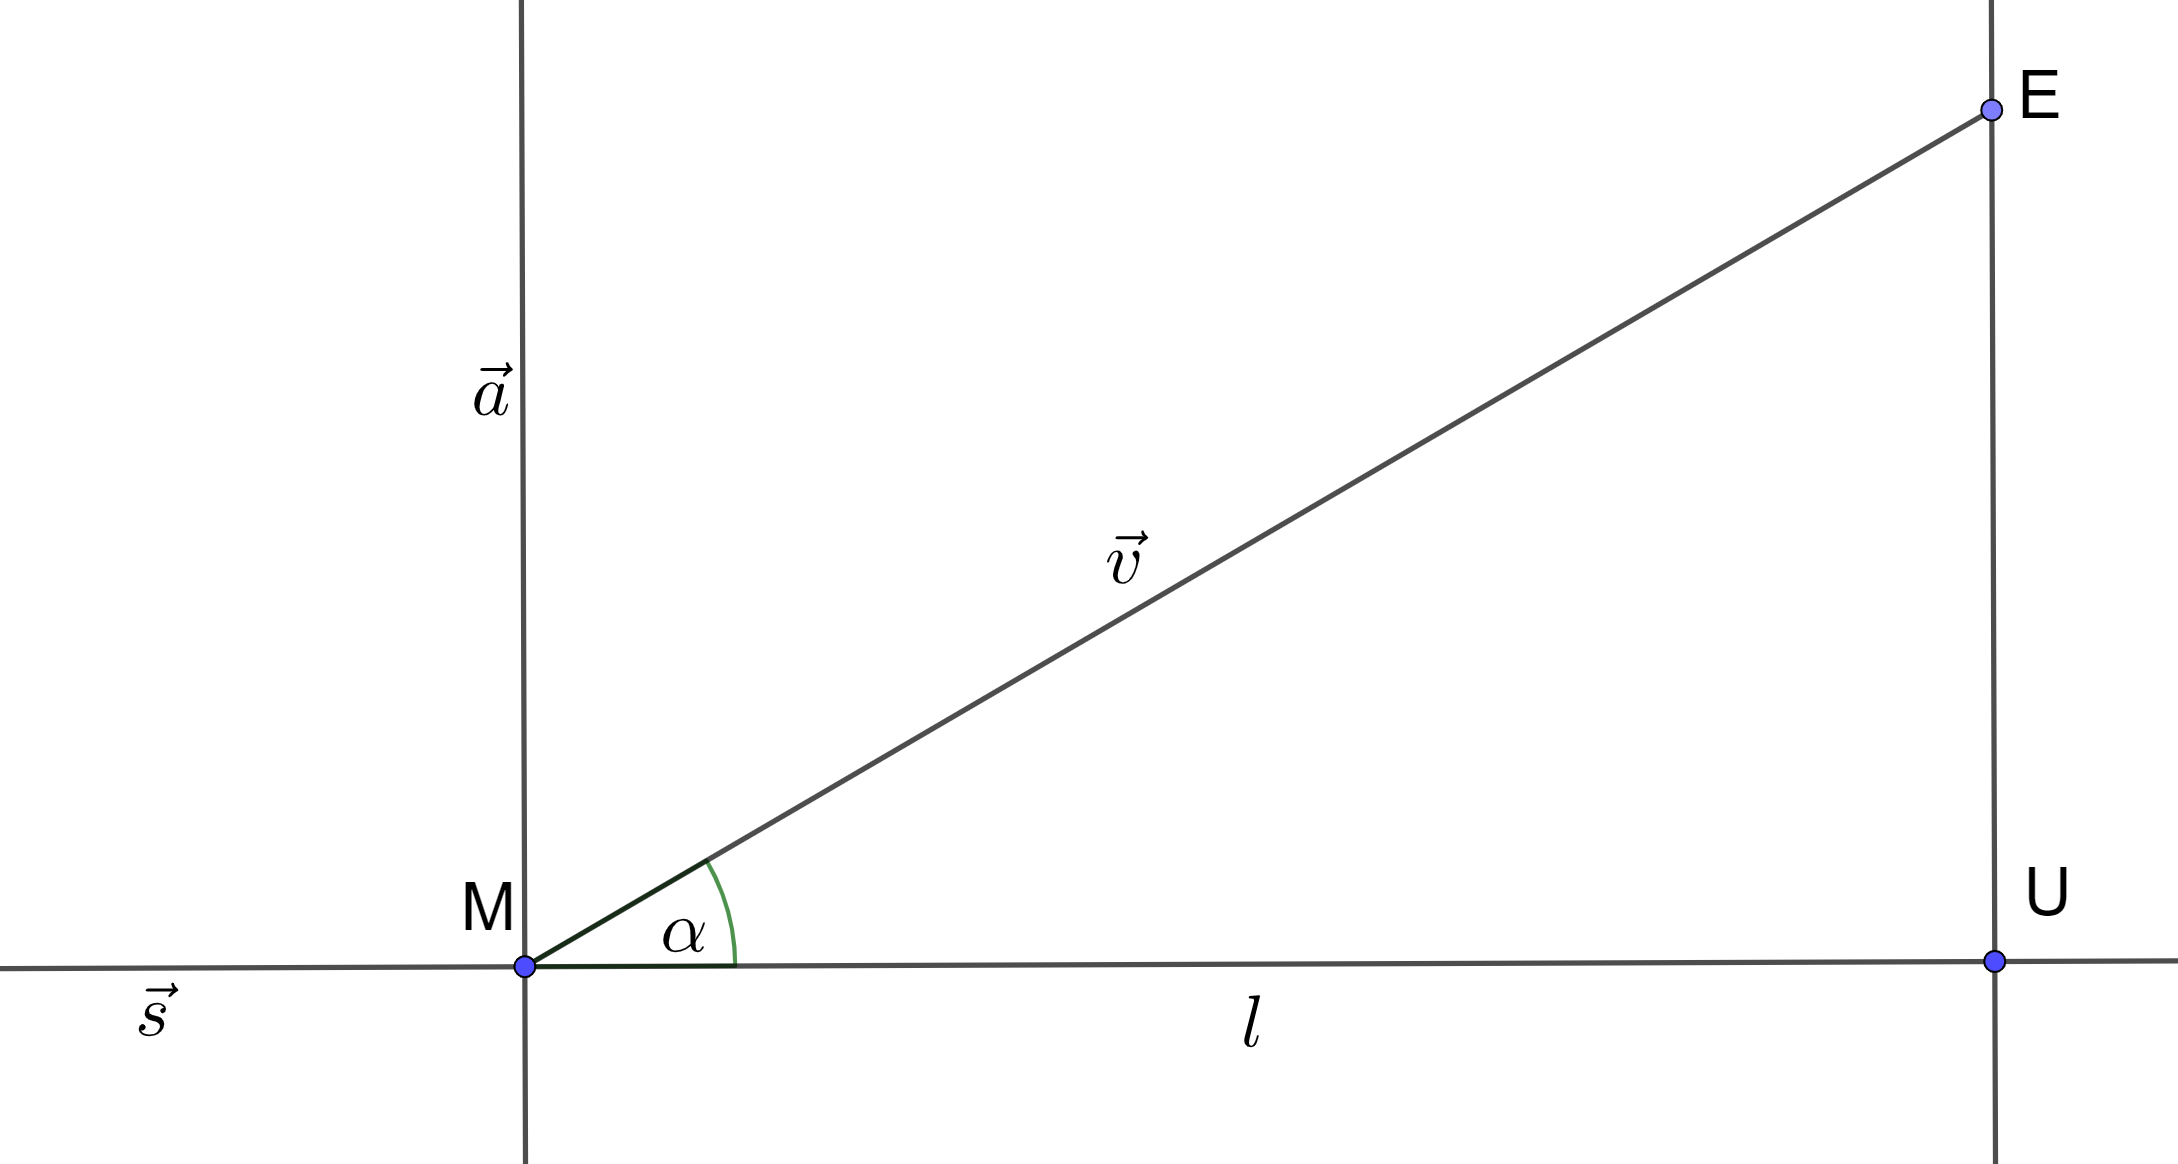
\includegraphics[width=.75\textwidth]{fig/Bildschirm_Skizze.png}
    \caption{Skizze für Auftreffen auf Bildschirm (mit GeoGebra erzeugt)}
    \label{fig:Schirm}
\end{figure}

%\subsection{Die geometrische Formel:}

%\subsection{Erklärung/Umsetzung der Physik im Code:}

Für die Umsetzung der obigen Formeln im Code wird wie folgt vorgegangen. 
Bei der Berechnung des Winkels $\alpha$ wird der arctans der oben bereits genannten Formel (\ref{eq:tan}) genommen und mit zwei multipliziert, da auf der Ausgabe der tatsächliche Winkel $\alpha$ zu sehen sein soll.
Der Winkel $\alpha$ wird im Bogenmaß berechnet, aber später in Grad ausgegeben.
Bei der \lstinline$Ablenkungsrichtung$ wird der Richtungsvektor des Strahl mit $-1$ multipliziert und danach das Kreuzprodukt mit dem Richtungsvektor des Ablenkspulenpaars gebildet, wie bereits in Formel (\ref{eq:a}) genannt.
Durch den Ausdruck \lstinline$this.richtungsvektor$ wird auf den Richtungsvektor des jeweiligen Magnetfeldes verwiesen.
Des Weiteren ist noch hinzuzufügen, dass die Berechnung jedes Ablenkspulenpaar für sich macht und daher auch eigene Werte für \lstinline$alpha$, den \lstinline$Bahnradius$ und die \lstinline$Ablenkungsrichtung$ hat.
Durch die Schleife wird bewirkt, dass wie oben bereits genannt die Berechnung des \lstinline$Ergebnisvektors$ für jedes der Spulenpaare gemacht wird.
Dies bedeutet, dass auf den \lstinline$Ergebnisvektor$, welcher zu Beginn auf den \lstinline$Bildschirmabstand$ als $x$-Koordinate, $0$ als $y$-Koordinate und 0 als $z$-Koordinate gesetzt ist, erst die Formel (\ref{eq:v_d}) benutzt wird und addiert wird.
Danach wird die Formel (\ref{eq:v_d}) erneut benutzt und erneut addiert. Dies führt dazu, dass der Punkt $E$ auf dem Schirm nun berechnet ist.

\begin{lstlisting}
alpha = 2 * Math.atan(felddurchmesser / (2 * bahnradius));

ablenkungsrichtung
  = strahl.quelle.richtungsvektor.
    multiplizieren(-1).
    kreuzprodukt(this.richtungsvektor);

Vektor ergebnisvektor = new Vektor(bildschirmabstand,0,0);
for (Ablenkspulenpaar m : getWorld().getObjects(Ablenkspulenpaar.class))
{
    ergebnisvektor
        = ergebnisvektor.addieren(m.ablenkungsrichtung.
          multiplizieren(bildschirmabstand * Math.tan(m.alpha)));
}
return ergebnisvektor;
\end{lstlisting}

Die Umrechnung des dreidimensionalen Ergebnisvektors (und aller anderen verwendeten 3D-Punkte und Vektoren) auf die Bildschirmebene des Programms wird in Anhang \ref{sec:lin} erläutert.
%\begin{tabular}{c|c|c}
    % Formel Buch & Formel Block & Anmerkungen  \\
     %\hline
    %$\alpha = \frac{d}{r}$ &$\tan(\frac{\alpha}{2}) = \frac{d}{2\cdot r}$& wegen Kleinwinkelnäherung bei dem Buch \\
    %\hline
   %$r = \frac{m\cdot v}{q\cdot B}$  & $r = \frac{m\cdot v}{q\cdot B}$& alles gleich 
     
%\end{tabular}
